\documentclass[a4paper,twoside,flushend, 10pt]{article}
\usepackage{times}
\usepackage{ijfis-scopus}
\usepackage{color}
\usepackage{epsfig, picins}
\usepackage{paralist}
\usepackage{cite}
\usepackage{algorithmic}
\usepackage{textcomp}
\usepackage{xcolor}
\usepackage{amsthm}
\usepackage{mathabx}
\usepackage{caption}
\usepackage{tablefootnote}
\usepackage{array}
\usepackage{mathrsfs}
\usepackage{kotex}
\usepackage{float}
\usepackage{multirow}
\usepackage{colortbl}
\usepackage{booktabs}
\usepackage{xcolor}
\usepackage{xpatch}
\usepackage{amsmath, amssymb, mathtools, color, graphicx, hyperref}
\usepackage[microtype]{letterspace}
%===========================================================

\begin{document}

\title{Hybrid multimodal GenAI for solving math problems containing various figures}

\author{Sangsoo Lee\inst{1}\inst{2}, Jae-Hyun Baek\inst{1}\inst{2}, Jon-Lark Kim\inst{1}\inst{2}\inst{3}}

\institute{
\inst{1}Department of Mathematics, Sogang University, Seoul, Korea
\\
\inst{2}Institute for Mathematical and Data Sciences, Sogang University, Seoul, Korea
\\
\inst{3}DeepFountain Corp., Seoul, Korea
}

\begin{abstract}
We propose a hybrid approach that combines OpenMath-Instruct-2 generative AI model for creating synthetic math problems—with ColPali, which employs Vision Language Models for document retrieval. By testing this system on the multimodal MathVision dataset, our method significantly outperformed traditional OCR-based solutions, particularly in interpreting graphs and bar charts. Notably, when applied to 58 statistical problems, accuracy jumped from 0\% (using OCR alone) to 29.3\% with the integration of ColPali and LLaMA and 62.1\% with the integration of ColPali and GPT-4o. These findings open up promising avenues for AI-driven solutions in education and data analysis.
\end{abstract}

\begin{keyword}
Generative AI, multimodal reasoning, vision language models, mathematical problem solving
\end{keyword}

\maketitle
\runningtitle{2025}{}{}{}{}{Sangsoo Lee, Jae-Hyun Baek and Jon-Lark Kim}{}
\makefoot{}{}{}{Jon-Lark Kim}{jlkim@sogang.ac.kr}{8}\hspace{0.5cm}
\begin{minipage}[t]{13cm}
%===========================================================
\section{Introduction}
Mathematical reasoning with visual components remains a significant challenge in the rapidly evolving field of AI. While NLP and computer vision have advanced considerably, integrating these modalities for mathematical problem-solving is still difficult. Traditional OCR systems often fail to capture the intricate relationships between text and visual elements, especially in graphs, diagrams, and mathematical charts.

Recent advancements in generative AI offer promising solutions. OpenMathInstruct-2\cite{TDM2024}, using the LLaMA framework\cite{DJP2024}, generated 14 million synthetic question-answer pairs, demonstrating strong mathematical reasoning capabilities. Similarly, ColPali\cite{FSW2024} leverages Vision Language Models (VLMs) to enhance document understanding by processing text and visuals together. These models show potential in bridging the gap in visually grounded mathematical tasks.

The contributions of this paper are twofold: (1) We propose a novel hybrid system combining OpenMathInstruct-2 and ColPali, demonstrating significant improvements in multimodal mathematical reasoning on the MathVision dataset\cite{WPS2024}; (2) We achieve a performance leap in statistical reasoning, increasing accuracy from 0\% to 29.3\% with our integrated model and further to 62.1\% when incorporating GPT-4o. These results contribute to more effective AI-driven mathematical problem-solving, with practical applications in educational technologies.


\end{minipage}
\newpage
\section{Literature review}
\noindent
The transformative journey of modern artificial intelligence began with the seminal work of Vaswani et al. \cite{VSP17} in 2017, which revolutionized natural language processing through the introduction of the Transformer architecture. This breakthrough laid the foundation for today's large language models and mathematical reasoning systems, marking a paradigm shift in how AI processes and understands information.

\begin{figure}[H]
    \centering
    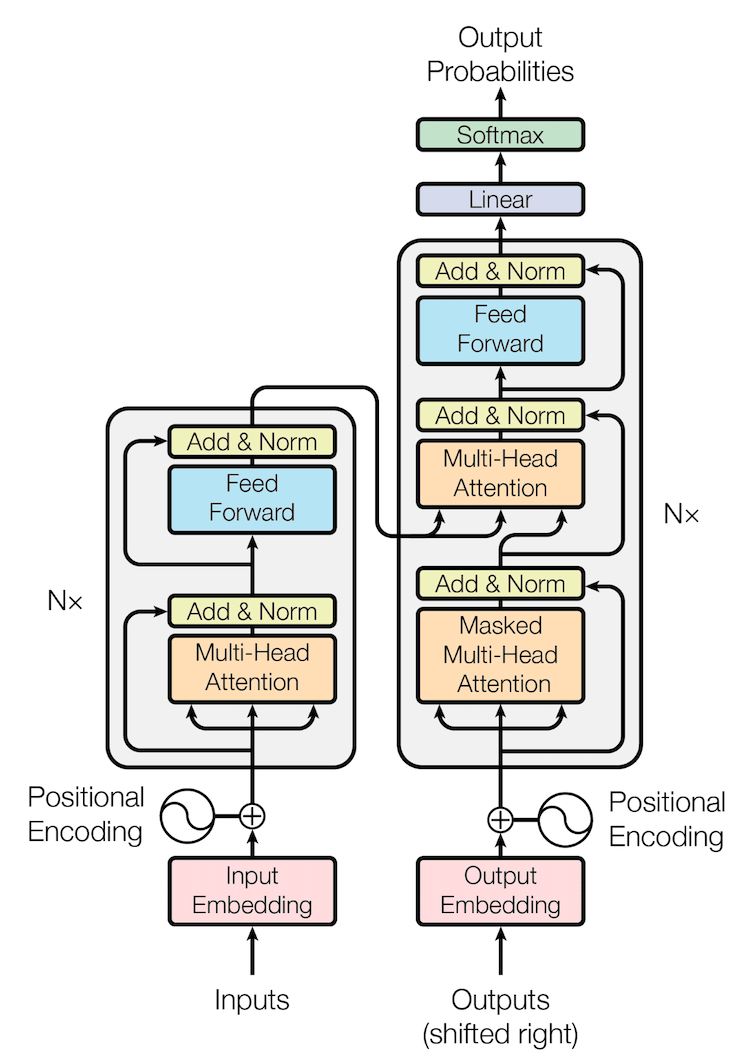
\includegraphics[width=65mm]{transformer.png}
    \caption{Transformer's self-attention mechanism}
    \label{fig:transformer}
\end{figure}

Building on this foundation, OpenMathInstruct-2 \cite{TDM2024} has pushed the boundaries of mathematical reasoning capabilities. Through an innovative teacher-student paradigm, the system generated 14 million synthetic question-answer pairs, including 600,000 unique problems. This approach yielded remarkable results, demonstrating a 7.8\% accuracy improvement in mathematical reasoning tasks. The implementation of Chain-of-Thought (CoT) reasoning further enhanced performance on challenging benchmarks like GSM8K and MATH by 3.9\%, while expanding question diversity from 1,000 to 6,500 led to a 10.5\% improvement in generalization capabilities.

ColPali \cite{FSW2024} represents a breakthrough in multimodal document understanding, building upon earlier work in efficient passage search techniques \cite{KZ2020}. Unlike traditional OCR-based approaches like Tesseract \cite{S2007}, ColPali employs a novel late interaction mechanism that computes token-level similarities between query and document embeddings, enabling nuanced interpretation of complex visual and textual elements.

The MathVision dataset \cite{WPS2024} has emerged as a crucial benchmark for evaluating multimodal mathematical reasoning systems. Its diverse collection of problems, spanning algebra, geometry, and statistics, presents unique challenges that test the limits of current AI capabilities. The dataset's emphasis on visual reasoning, particularly in statistical problems, has proven instrumental in validating the effectiveness of integrated approaches like those proposed by Jiang et al. \cite{JXA2020} for probing model knowledge.

Recent advances in prompt engineering, exemplified by Zhou et al.'s Context Optimization (CoOp) \cite{ZYL2022}, have transformed how vision-language models interact with diverse inputs. By replacing static prompts with trainable context vectors, CoOp achieved up to 45\% accuracy improvements in few-shot learning scenarios. This adaptive approach has proven particularly effective in handling domain shifts, as demonstrated on challenging datasets like ImageNet-Sketch and ImageNet-R.

CLIP's \cite{RKH2021} groundbreaking approach to aligning visual and textual embeddings has set new standards for multimodal understanding. Through contrastive learning, CLIP successfully bridges the gap between visual and linguistic representations, enabling zero-shot transfer across diverse tasks. This unified embedding approach has become fundamental to modern multimodal AI systems, as demonstrated in recent tool-integrated reasoning approaches \cite{GSG2024}.

The integration of these technologies has opened new frontiers in AI-driven mathematical problem-solving. By combining ColPali's multimodal retrieval capabilities with LLaMA's advanced reasoning framework \cite{DJP2024}, our approach achieves unprecedented accuracy in handling complex mathematical problems. The system's ability to process both visual and textual information simultaneously represents a significant step forward in artificial intelligence, particularly in educational technology and automated reasoning applications.

These developments collectively point toward a future where AI systems can seamlessly integrate visual and textual understanding in mathematical reasoning tasks. While challenges remain in scaling these solutions and ensuring robust performance across diverse problem domains, the foundation has been laid for continued innovation in this rapidly evolving field.


\section{Hybrid multimodal mathematical problem-solving framework}
\noindent
To solve multimodal mathematical problems, this study adopts a hybrid methodology that combines the strengths of three core approaches: traditional OCR-based retrieval, ColPali's Vision Language Model (VLM)-based retrieval, and LLaMA's reasoning capabilities. Together, these methods enable robust processing and integration of textual and visual components, ensuring accurate and efficient solution generation.

The OCR-based retrieval serves as the foundation for handling text-heavy problems. OCR tools extract and segment textual content from document images, identifying layout elements such as paragraphs, tables, and figures. This text is embedded into a feature space using a text embedding model, enabling efficient similarity-based retrieval\cite{FSW2024}. However, OCR's reliance on textual data limits its applicability to problems requiring visual understanding, such as interpreting diagrams or graphs. Figure~\ref{fig:ocr_pipeline} illustrates this workflow.

\begin{figure}[H]
    \centering
    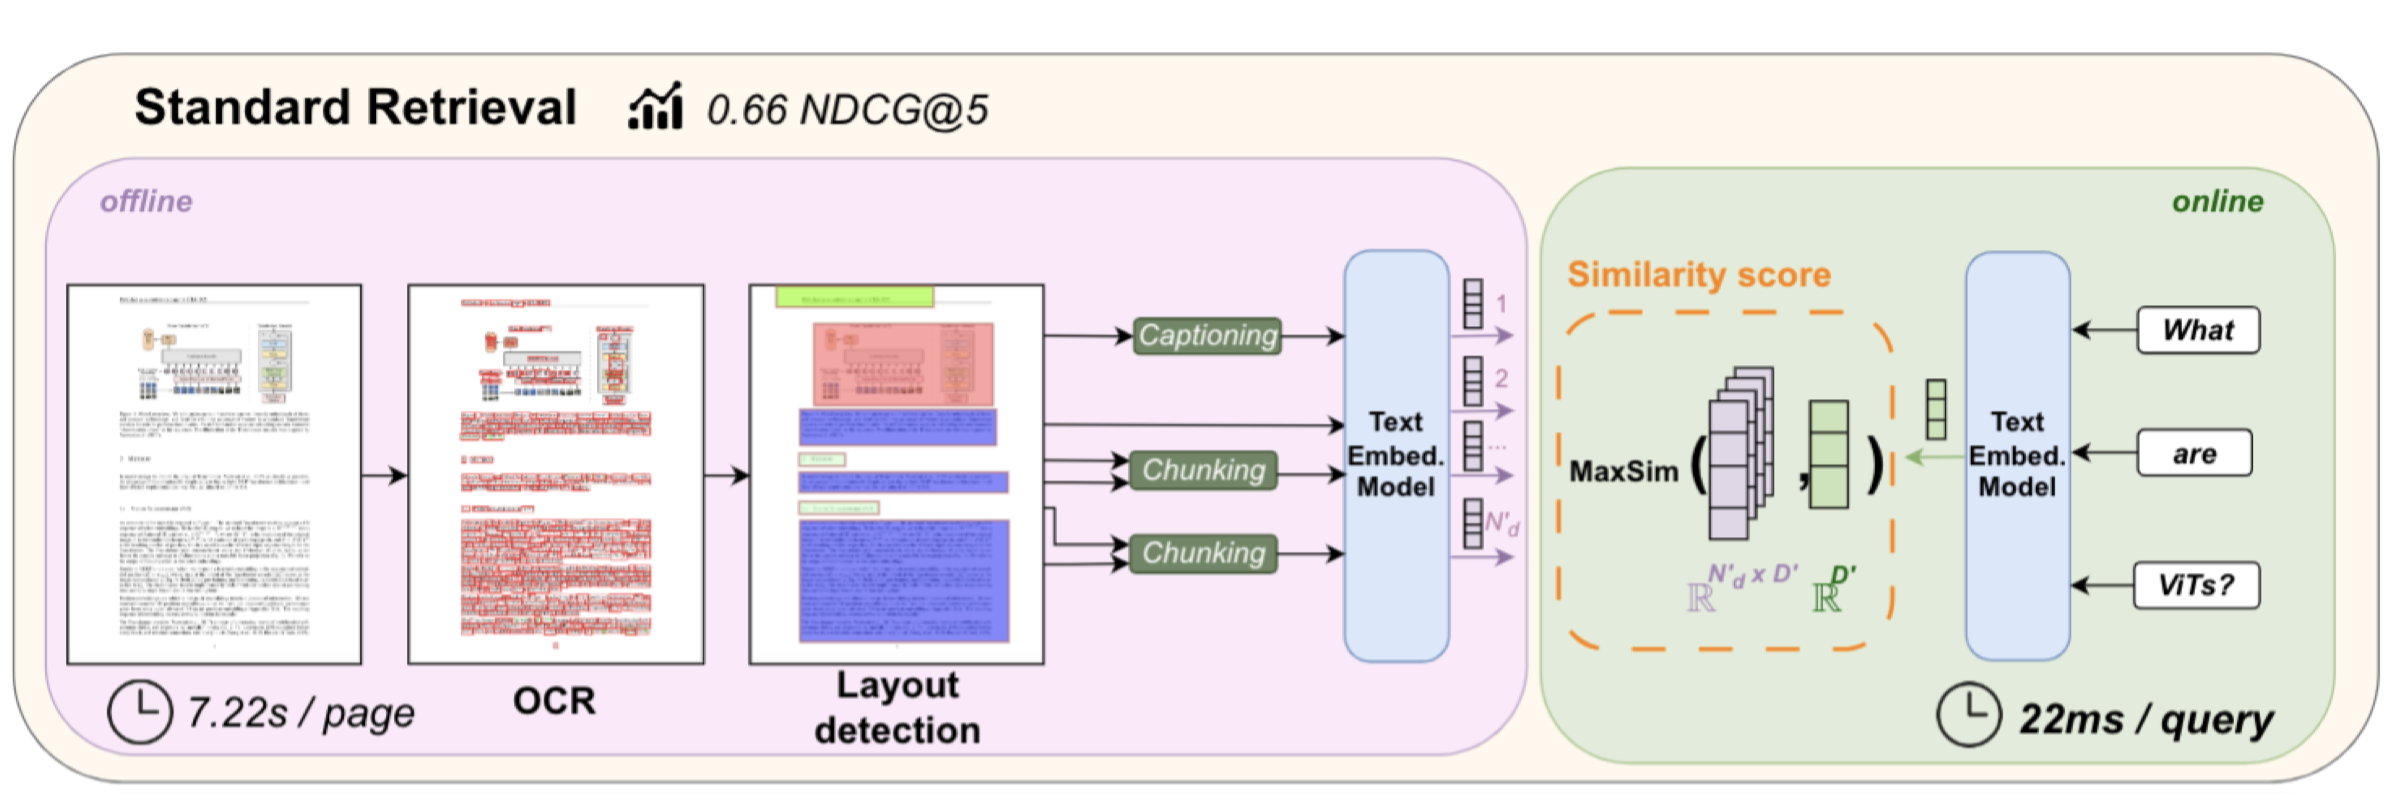
\includegraphics[width=85mm]{ocrfigure.png}
    \caption{Workflow of the OCR-based retrieval method.}
    \label{fig:ocr_pipeline}
\end{figure}

To address these limitations, ColPali leverages Vision Language Models (VLMs) to process both textual and visual information. A Vision Encoder extracts visual features, while a Large Language Model (LLM) processes the textual content. Both are projected into a shared embedding space, enabling multimodal understanding\cite{FSW2024}. Figure~\ref{fig:colpali_pipeline} shows the ColPali retrieval workflow, which includes token-level similarity matching through a late interaction mechanism. This allows ColPali to retrieve solutions even for visually complex problems, such as those involving bar graphs or statistical charts, where OCR struggles\cite{FSW2024}.

\begin{figure}[H]
    \centering
    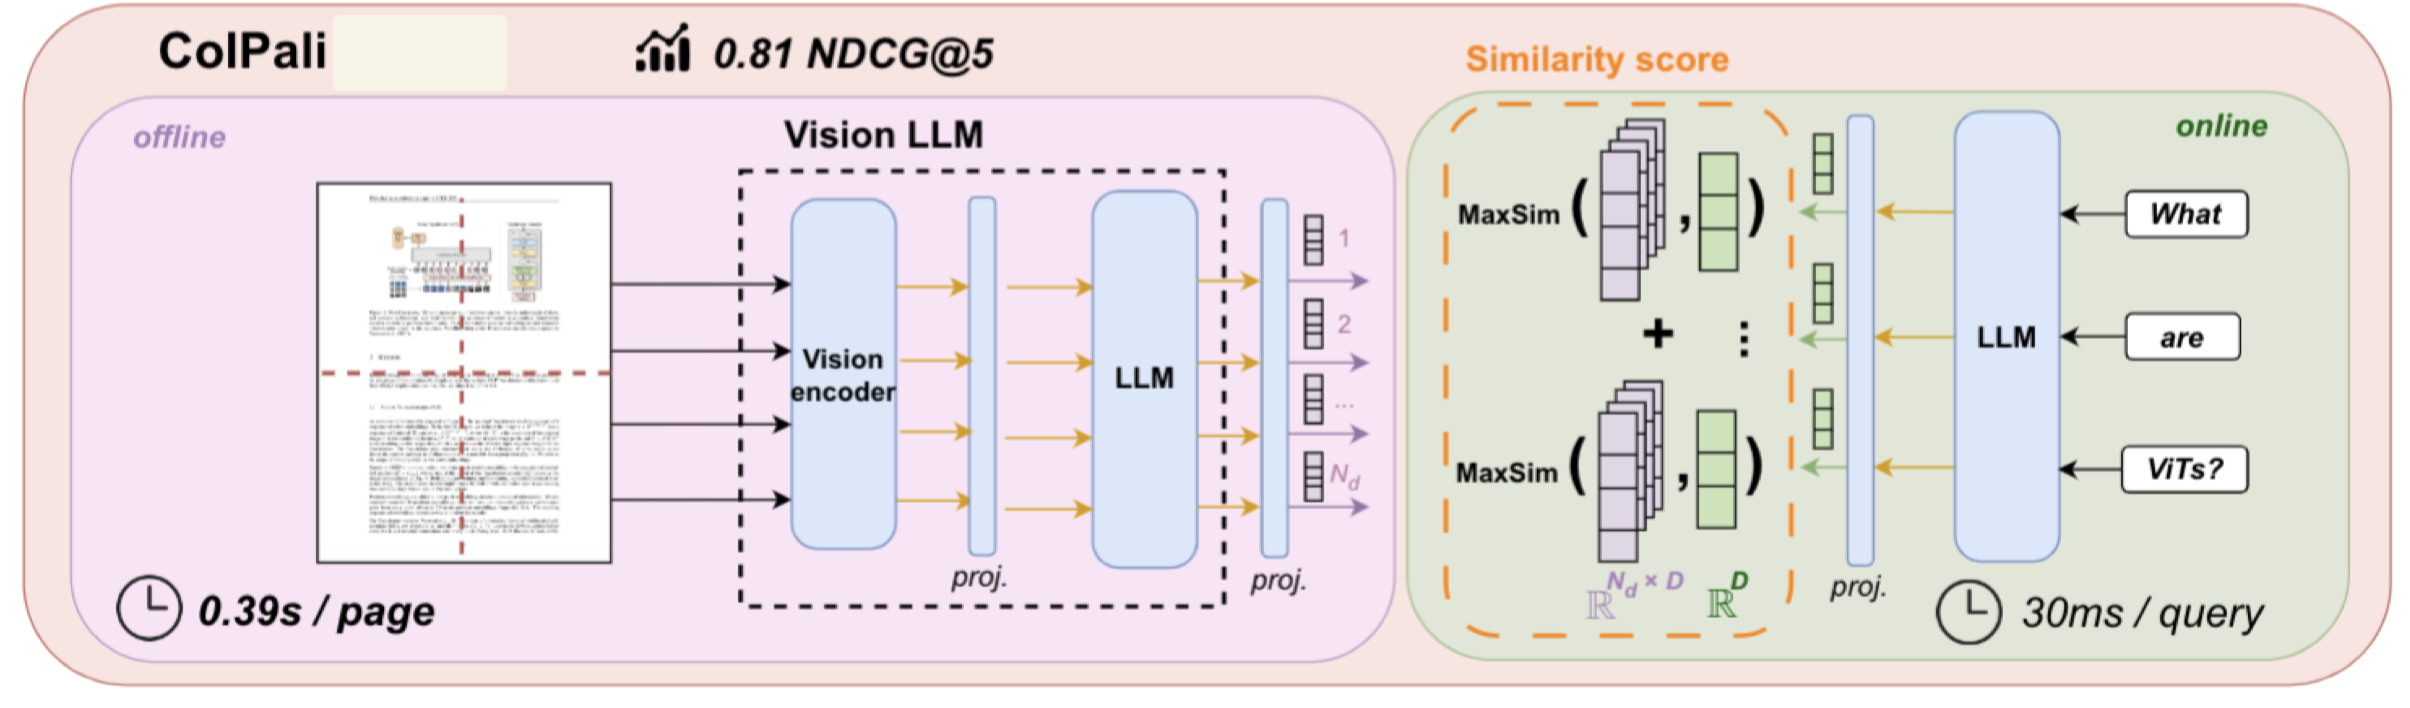
\includegraphics[width=85mm]{colpalifigure.png}
    \caption{Workflow of the ColPali retrieval method.}
    \label{fig:colpali_pipeline}
\end{figure}

LLaMA complements these retrieval methods by providing advanced reasoning capabilities. Using datasets fine-tuned for mathematical problem-solving, LLaMA excels at generating step-by-step solutions through its Chain-of-Thought (CoT) methodology\cite{TDM2024}. This enables logical deduction and reasoning across both text-dominant and multimodal problems. In this hybrid system, LLaMA integrates seamlessly with OCR and ColPali, transforming retrieved data into comprehensive and interpretable solutions.

Table~\ref{tab:ndcg_comparison} compares the NDCG@5 scores of OCR-based and ColPali methods across different categories. While OCR performs well for text-only documents, ColPali demonstrates superior accuracy in handling multimodal content, showcasing the necessity of integrating visual understanding into the retrieval pipeline\cite{FSW2024}.

\begin{table}[H]
    \centering
    \renewcommand{\arraystretch}{1.3}
    \caption{NDCG@5 comparison for OCR-based and ColPali methods across document categories.}    
    \begin{tabular}{>{\columncolor{gray!10}}p{3.2cm}>{\centering}p{2.3cm}>{\centering\arraybackslash}p{2.3cm}}
        \toprule
        \rowcolor{gray!20}
        \textbf{Category} & \textbf{OCR-Based NDCG@5} & \textbf{ColPali NDCG@5} \\
        \midrule
        Text-Only & 0.78 & 0.79 \\
        Text with Visuals & 0.58 & \textbf{0.76} \\
        Rich Visual Content & 0.31 & \textbf{0.68} \\
        \bottomrule
    \end{tabular}

    \label{tab:ndcg_comparison}
\end{table}

This hybrid system optimally combines the strengths of OCR, ColPali, and LLaMA. OCR provides a robust baseline for text-dominant problems, ColPali expands the system's capabilities to handle multimodal inputs, and LLaMA ensures logical and interpretable solution generation\cite{TDM2024}. In the following section, we detail the experimental setup, evaluation metrics, and results that demonstrate the effectiveness of this approach in solving multimodal mathematical problems.

\section{Experiments}
\noindent
The experiments aimed to evaluate the performance of the proposed ColPali-based approach in solving multimodal mathematical problems, with a focus on the MathVision dataset. To benchmark its capabilities, ColPali was compared against the OCR-based approach and GPT series(4o, o1), both using the LLaMA model as the reasoning backbone\cite{WPS2024, FSW2024, TDM2024}.

\subsection{Experimental setup}
\noindent
Our evaluation framework incorporated two distinct datasets. MathVision, a comprehensive collection of approximately 70,000 problems spanning both text-based and image-based categories, provided a robust testbed for multimodal analysis. We specifically focused on its "Statistics" category, which comprises 58 visually complex problems, to rigorously evaluate the models' capacity for interpreting integrated textual and visual elements\cite{WPS2024}. Additionally, we leveraged GSM8K, an established dataset containing 8,000 high-quality word problems, to benchmark the fundamental reasoning capabilities and guide our model selection process\cite{TDM2024}.

\begin{table}[H]
    \centering
    \footnotesize
    \renewcommand{\arraystretch}{1.3}
    \caption{Comparison of the GSM8K and MathVision datasets.}
    \begin{tabular}{>{\columncolor{gray!10}}p{1.8cm}p{2.8cm}p{2.8cm}}
        \toprule
        \rowcolor{gray!20}
        \textbf{Dataset} & \textbf{Scope} & \textbf{Purpose} \\
        \midrule
        GSM8K & Text-based logical reasoning & Benchmark reasoning performance \\
        MathVision & Multimodal (text and image) problems & Evaluate multimodal capabilities \\
        \bottomrule
    \end{tabular}
    \label{tab:dataset_comparison}
\end{table}

To rigorously evaluate the proposed framework's reasoning and multimodal problem-solving capabilities, we strategically employed two complementary datasets: GSM8K and MathVision. This dual-dataset approach enabled comprehensive assessment across both traditional reasoning tasks and complex multimodal scenarios, as summarized in Table~\ref{tab:dataset_comparison}.

The GSM8K dataset, comprising 8,000 meticulously curated word problems, represents a gold standard for evaluating mathematical reasoning capabilities\cite{TDM2024}. These problems, spanning arithmetic, geometry, and algebraic domains, are specifically designed to assess step-by-step logical deduction and solution synthesis. We leveraged this dataset as a critical benchmark for evaluating the fundamental reasoning capabilities of our models, particularly LLaMA, GPT-4o, and GPT-o1 thereby establishing a robust foundation for our reasoning architecture selection.

For multimodal evaluation, we employed the MathVision dataset\cite{WPS2024}, an extensive collection encompassing approximately 70,000 diverse mathematical problems. This dataset's unique strength lies in its comprehensive coverage of both text-centric and image-integrated problem scenarios. Our investigation specifically focused on the Statistics subset, consisting of 58 sophisticated problems characterized by complex visual elements such as statistical graphs and data visualizations. These problems presented an ideal testbed for evaluating ColPali's Vision Language Models (VLMs), as they demanded sophisticated integration of visual interpretation and mathematical reasoning\cite{FSW2024}. This careful selection enabled us to rigorously assess the framework's capacity for real-world multimodal problem-solving.

While GSM8K provided a robust benchmark for reasoning capabilities, MathVision served as the primary dataset to evaluate multimodal problem-solving. By combining these datasets, the study ensured a comprehensive assessment of both text-based and visual reasoning abilities.

In this study, we conducted a comprehensive comparison of three distinct models. The first model combines OCR-based text extraction with LLaMA for reasoning, though this approach is inherently limited by its reliance on textual input alone when handling problems with visual components\cite{FSW2024}. The second model integrates ColPali's Vision Language Models (VLMs) with LLaMA, enabling sophisticated multimodal reasoning through simultaneous processing of visual and textual data\cite{FSW2024}. Finally, we employed GPT-4o and o1, proprietary large language models, as our baseline for comparative analysis\cite{WPS2024}.


\subsection{Comparative analysis of visual problem-solving approaches}
\noindent

We evaluated four distinct approaches: OCR-based, ColPali, GPT-4o and o1 on representative visual mathematical problems from MathVision. Here we present detailed analyses of their performance on three key examples.

\medskip

\textbf{Problem 1:} Given the gas price data shown in Figure~\ref{fig:gas_prices}, calculate the percentage difference between the highest and lowest prices.

\begin{figure}[H]
    \centering
    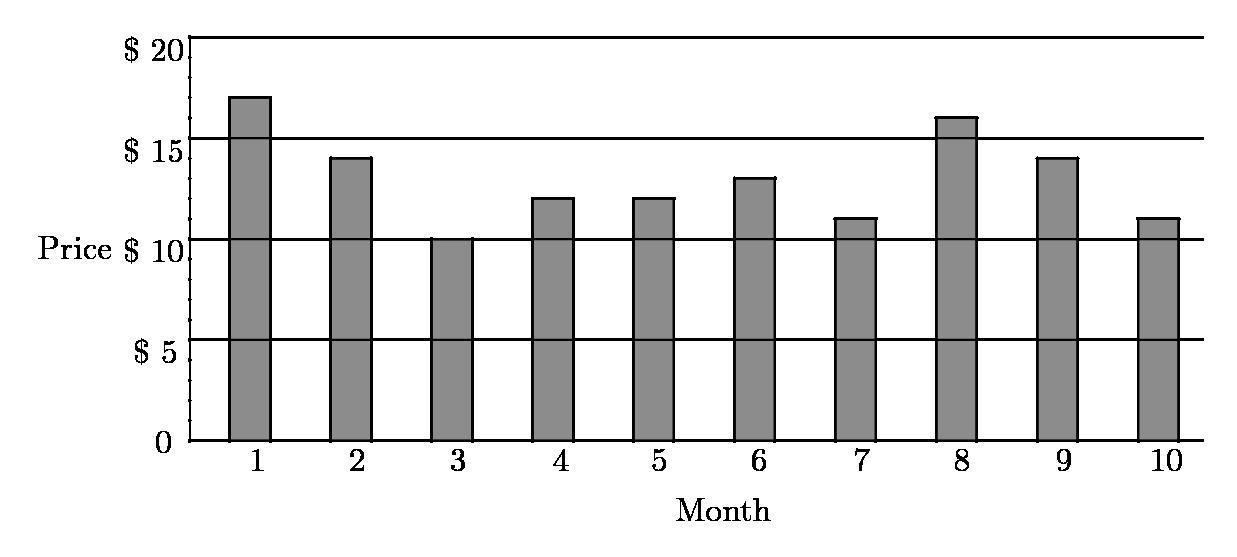
\includegraphics[width=0.45\textwidth]{gas_prices.jpg}
    \caption{Bar graph showing gasoline prices over time}
    \label{fig:gas_prices}
\end{figure}

\begin{table}[H]
    \centering
    \footnotesize
    \caption{Gas price analysis results}
    \begin{tabular}{>{\columncolor{gray!10}}p{1.2cm}p{1.2cm}p{1.2cm}p{1.9cm}}
        \toprule
        \rowcolor{gray!20}
        \textbf{Step} & \textbf{OCR} & \textbf{GPT-o1} & \textbf{ColPali+LLaMA} \\
        \midrule
        Max & \$20 & \$18 & \textbf{\$17} \\
        Min & \$0 & \textbf{\$10} & \textbf{\$10} \\
        Result & 200\% & 80\% & \textbf{70\%} \\
        \bottomrule
    \end{tabular}
    \label{tab:gas_results}
\end{table}

As shown in Table~\ref{tab:gas_results}, the OCR-based approach demonstrated significant limitations in price value extraction, erroneously identifying a maximum of \$20 and a minimum of \$0, leading to an unrealistic difference calculation of 200\%. In contrast, ColPali exhibited superior visual data processing capabilities by accurately identifying the maximum price of \$17 and minimum price of \$10, resulting in a precise price difference calculation of 70\%. This stark contrast in performance clearly illustrates ColPali's superior capability in handling visual data compared to the conventional OCR-based approach, particularly in scenarios requiring precise numerical extraction and interpretation.

\medskip

\textbf{Problem 2:} Based on the color preference survey data presented in Figure~\ref{fig:color_preferences}, determine the percentage of respondents who indicated blue as their preferred color.

\begin{figure}[H]
    \centering
    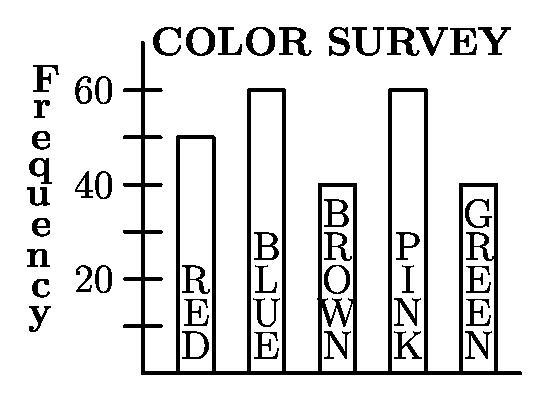
\includegraphics[width=0.35\textwidth]{color_survey.jpg}
    \caption{Distribution of color preferences from survey respondents (n=250)}
    \label{fig:color_preferences}
\end{figure}

\begin{table}[H]
    \centering
    \caption{Comparative analysis of color preference interpretation}
    \begin{tabular}{>{\columncolor{gray!10}}p{2.5cm}p{4.5cm}}
        \toprule
        \rowcolor{gray!20}
        \textbf{Model} & \textbf{Analysis Process} \\
        \midrule
        GPT-4o 
        & \textit{Data Extraction:} Red(50), Blue(60), Brown(40), Pink(60), Green(20) \\
        & \textit{Computation:} $\tfrac{60}{200}\times 100 = 30\%$ \\
        \midrule
        GPT-o1 
        & \textit{Data Extraction:} Red(50), Blue(60), Brown(30), Pink(60), Green(40) \\
        & \textit{Computation:} $\tfrac{60}{240}\times 100 = 25\%$ \\
        \bottomrule
        ColPali + LLaMA
        & \textit{Data Extraction:} \textbf{Red(50), Blue(60), Brown(40), Pink(60), Green(40)} \\
        & \textit{Computation:} $\tfrac{60}{250}\times 100 = 24\%$ \\
        \midrule
    \end{tabular}
    \label{tab:color_analysis}
\end{table}


Looking at Table~\ref{tab:color_analysis}, the analysis reveals critical insights into the capabilities and limitations of both models in processing visual data. While both models successfully identified the frequency of blue preferences (60), their overall performance differed significantly. GPT series' misidentification of the green category frequency (reporting 20 instead of 40) points to potential weaknesses in distinguishing similar visual elements or handling data in certain color ranges. This error cascaded into a more serious analytical mistake - an incorrect total population count of 200 instead of 250, leading to a substantially overestimated percentage of 30\%. In contrast, ColPali exhibited remarkable precision in visual data extraction across all color categories, accurately identifying each frequency value and computing the correct proportion of 24\%. This performance gap not only highlights ColPali's superior visual processing capabilities but also emphasizes the importance of accurate base data extraction for reliable statistical analysis. The results suggest that ColPali's architecture may be better suited for real-world applications where precise visual data interpretation is crucial for decision-making processes.

\medskip

\textbf{Problem 3:} Using the grade distribution shown in Figure~\ref{fig:grades}, determine the proportion of satisfactory grades (A-D).

\begin{figure}[H]
    \centering
    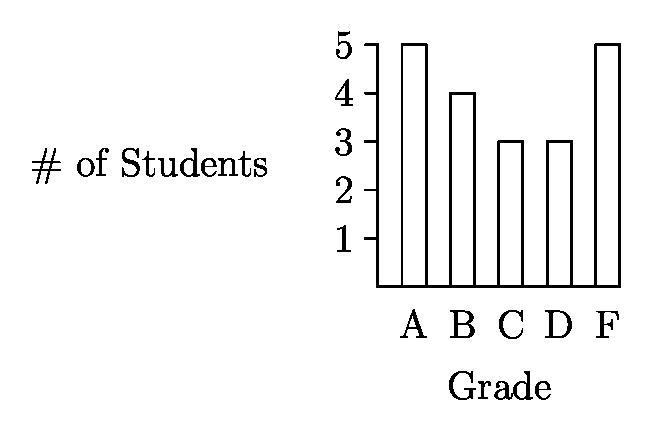
\includegraphics[width=0.35\textwidth]{grades.jpg}
    \caption{Grade distribution histogram}
    \label{fig:grades}
\end{figure}

\begin{table}[H]
    \centering
    \footnotesize
    \caption{Grade analysis results}
    \begin{tabular}{>{\columncolor{gray!10}}p{1.2cm}p{1.9cm}p{1.2cm}p{1.2cm}}
        \toprule
        \rowcolor{gray!20}
        \textbf{Step} & \textbf{ColPali+LLaMA} & \textbf{GPT-4o} & \textbf{GPT-o1} \\
        \midrule
        Count & \textbf{15/20} & 12/17 & 14/19\\
        Result & \textbf{0.750} & 0.706 & 0.737\\
        \bottomrule
    \end{tabular}
    \label{tab:grade_results}
\end{table}

The analysis of grade distribution calculations, as presented in Table~\ref{tab:grade_results}, reveals significant differences in model performance. ColPali exhibited exceptional accuracy in visual data processing, successfully identifying 15 out of 20 grades and calculating the precise proportion of 3/4 for satisfactory grades. This demonstrates its robust capability in handling complex visual information and performing accurate mathematical computations. In contrast, GPT-4o's performance showed notable limitations, with errors in both the fundamental counting process (identifying only 12 out of 17 grades) and subsequent calculations (arriving at 0.706). This performance gap highlights a critical distinction in visual processing capabilities between the two models, with ColPali's architecture proving more reliable for educational assessment applications where precise grade analysis is essential. The results underscore the importance of accurate visual data extraction as a foundation for dependable statistical analysis in academic contexts.

\medskip

\textbf{Problem 4:} Given a total population of 480 and the ratio shown in Figure~\ref{fig:population}, determine the male population.

\begin{figure}[H]
    \centering
    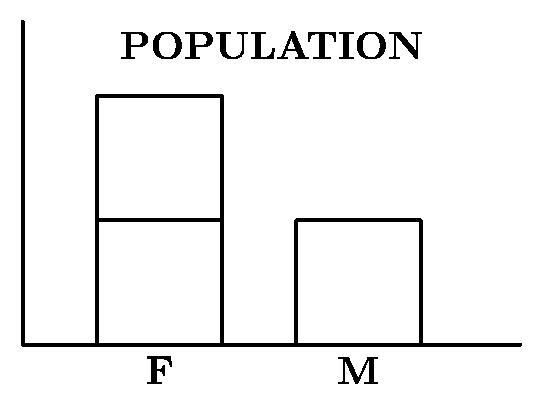
\includegraphics[width=0.35\textwidth]{population.jpg}
    \caption{Population distribution diagram}
    \label{fig:population}
\end{figure}

\begin{table}[H]
    \centering
    \caption{Population analysis steps and results}
    \begin{tabular}{>{\columncolor{gray!10}}p{3cm}p{4cm}}
        \toprule
        \rowcolor{gray!20}
        \textbf{Step} & \textbf{ColPali+GPT-4o} \\
        \midrule
        Visual Extraction & Female:Male ratio = 2:1 \\
        Parts Analysis & Total parts = 3 \\
        Equation Setup & $3x = 480$ \\
        Final Result & Male population = 160 \\
        \bottomrule
    \end{tabular}
    \label{tab:population_analysis}
\end{table}

The integrated ColPali+GPT-4o approach, as detailed in Table~\ref{tab:population_analysis}, demonstrated remarkable superiority over the standalone GPT-4o model, particularly in handling the nuanced task of ratio extraction from visual data. While GPT-4o exhibited strong mathematical reasoning capabilities in abstract problem-solving, its limitations in processing visual information became evident in this specific case. The collaborative system leveraged ColPali's specialized visual processing architecture to accurately interpret the population ratio diagram, while GPT-4o's advanced language modeling capabilities enabled sophisticated mathematical reasoning on the extracted data. This synergistic combination not only solved the immediate problem but also highlighted a crucial insight: the future of complex mathematical problem-solving lies in the strategic integration of specialized visual processing systems with advanced language models. The success of this hybrid approach suggests a promising direction for developing more robust and versatile AI systems capable of handling real-world mathematical challenges that frequently span multiple modalities of information.

\subsection{Performance summary}

Table~\ref{tab:mathvision_results} summarizes the performance of the four models on the MathVision dataset, specifically focusing on the "Statistics" category. The accuracy is calculated based on the number of problems correctly solved out of the 58 problems in this category\cite{WPS2024}.

\begin{table}[H]
    \centering 
    \setlength{\tabcolsep}{10pt}
    \caption{Performance comparison on MathVision dataset (Statistics category)}
    \begin{tabular}{>{\columncolor{gray!10}}p{3cm}|>{\columncolor{gray!5}}p{1.8cm}|>{\columncolor{gray!5}}p{1.8cm}}
        \toprule
        \rowcolor{gray!20}
        \textbf{\large Model} & \textbf{\large Correct / Total} & \textbf{\large Accuracy (\%)} \\
        \midrule
        \textbf{OCR+LLaMA} & 0 / 58 & 0.0 \\
        \rowcolor{gray!10}
        \textbf{ColPali+LLaMA} & 17 / 58 & 29.3 \\
        \textbf{GPT-4o} & 31 / 58 & 53.4 \\
        \rowcolor{gray!10}
        \textbf{ColPali+GPT-4o} & \textbf{36 / 58} & \textbf{62.1} \\
        \bottomrule
    \end{tabular}
    \label{tab:mathvision_results}
\end{table}

The results clearly demonstrate the limitations of OCR-based methods, which failed to solve any problems due to their inability to interpret visual data. ColPali significantly outperformed OCR by solving 17 out of 58 problems correctly, achieving an accuracy of 29.3\%\cite{FSW2024}. GPT-4o achieved a higher accuracy of 53.4\%, demonstrating strong reasoning capabilities while still encountering challenges with complex visual elements\cite{WPS2024}.
The combined \textbf{ColPali + GPT-4o} approach demonstrated the best performance, solving 36 out of 58 problems with an accuracy of 62.1\%. This improvement highlights the synergy between ColPali's visual comprehension and GPT-4o's advanced reasoning abilities. ColPali effectively handled the extraction of visual data through multimodal embeddings and late interaction mechanisms, while GPT-4o provided the robust contextual reasoning that integrated and interpreted this extracted information.

        Analyzing the individual models, OCR-based methods failed due to their inability to handle visual elements like graphs and charts. ColPali outperformed OCR by integrating vision-language processing, yet faced challenges with ambiguous or noisy visuals. GPT-4o demonstrated strong textual reasoning skills but struggled with precise multimodal interpretation. In contrast, the hybrid \textbf{ColPali + GPT-4o} system bridged these gaps, showcasing the potential of combined approaches for complex multimodal reasoning tasks.
To further improve hybrid approaches, research should focus on enhancing ColPali’s visual token embeddings to better handle noisy or cluttered data. Deeper integration of visual and reasoning models could allow for more seamless end-to-end learning across text and image modalities. Additionally, expanding evaluations to include other categories like algebra and geometry will help test generalizability. Finally, adaptive fine-tuning strategies tailored to diverse problem formats should be explored to optimize performance.

\subsection{Discussion}
\noindent
The comparison demonstrates that OCR-based methods struggled to interpret essential visual elements, such as bar graphs, making them unsuitable for multimodal problems. ColPali’s ability to integrate visual and textual data allowed it to outperform OCR significantly. However, its limitations in reasoning through ambiguous visual structures indicate room for improvement. GPT-4o achieved higher overall accuracy compared to ColPali alone, but its struggles with precise multimodal reasoning highlight the need for more sophisticated visual understanding mechanisms. 

The combined \textbf{ColPali + GPT-4o} system achieved the highest accuracy by leveraging the complementary strengths of both models. ColPali’s visual comprehension enabled accurate data extraction from visual elements, while GPT-4o provided advanced reasoning to integrate and contextualize the extracted information. This collaboration demonstrates the potential of hybrid systems for tackling complex multimodal datasets like MathVision. Furthermore, ColPali’s open-source nature offers a promising alternative to proprietary systems, enabling broader access to advanced multimodal problem-solving capabilities in educational and research contexts.

In summary, the \textbf{ColPali + GPT-4o} combination highlights the feasibility and advantages of collaborative frameworks in solving complex mathematical problems. By bridging the gaps between visual comprehension and advanced reasoning, this approach sets a benchmark for future research in multimodal AI systems.

\section{Conclusion}
\noindent
This study evaluated a multimodal problem-solving framework by integrating ColPali's Vision Language Models (VLMs) with reasoning backbones like LLaMA and GPT-4o. By focusing on mathematical problems that require the interpretation of both visual and textual components, the framework demonstrated substantial improvements over OCR-based methods and offered competitive performance compared to standalone models. ColPali's enhanced multimodal understanding was evident in achieving a 29.3\% accuracy on the MathVision dataset's "Statistics" category, significantly outperforming the 0\% accuracy of OCR-based approaches\cite{WPS2024}. GPT-4o achieved a higher accuracy of 53.4\%, excelling in text-based reasoning tasks but still facing challenges with complex visual data. The hybrid \textbf{ColPali + GPT-4o} model achieved the best performance, with an accuracy of 62.1\%, demonstrating the effectiveness of combining robust visual comprehension with advanced reasoning capabilities\cite{FSW2024}. 

These findings highlight the complementary strengths and limitations of the different approaches. While ColPali excels in visual comprehension, it benefits from pairing with a powerful reasoning model like GPT-4o to handle more intricate problem-solving tasks. Conversely, GPT-4o\textquotesingle s strong reasoning skills are enhanced by ColPali\textquotesingle s ability to interpret the visual elements that pure text-based models find challenging. This synergy underscores the potential of hybrid frameworks in tackling real-world mathematical problems that frequently span multiple modalities.

Despite these advancements, further research is required. The experiments focused mainly on the "Statistics" category of the MathVision dataset, leaving other domains unexplored. Expanding to areas like Algebra, Geometry, and Calculus will provide a more comprehensive evaluation of generalizability. Moreover, improving computational efficiency and exploring end-to-end training strategies can help in creating more streamlined, adaptive systems. Enhancements in fine-tuning and adaptive multimodal embeddings could further improve performance across a diverse range of problem formats.

In conclusion, this study establishes a benchmark for the integration of vision-language comprehension and advanced reasoning in solving complex mathematical problems. By addressing current limitations and incorporating the latest advancements in model architectures, hybrid systems like \textbf{ColPali + GPT-4o} offer a promising path forward 
for AI-driven education, research, and data analysis.

\section*{Conflict of Interest}
\noindent
No potential conflict of interest relevant to this article was reported.

\section*{Acknowledgments}
\noindent
This research was supported by the BK21 FOUR (Fostering Outstanding Universities for Research) funded by the Ministry of Education(MOE, Korea) and National Research Foundation of Korea(NRF) with grant No.4120240415042.


\bibliographystyle{ieeetr}
\begin{thebibliography}{9}

\bibitem{VSP17}
A. Vaswani, N. Shazeer, N. Parmar, et al.,
``Attention is all you need,'' \emph{Advances in Neural Information Processing Systems}, Long Beach, CA, vol. 30, pp. 5998--6008, 2017.

\bibitem{TDM2024}
Toshniwal, S., Du, W., Moshkov, I., et al.,
``OpenMathInstruct-2: Accelerating AI for Math with Massive Open-Source Instruction Data,'' arXiv preprint arXiv:2410.01560, 2024.

\bibitem{FSW2024}
Faysse, M., Sibille, H., Wu, T., et al., 
``ColPali: Efficient Document Retrieval with Vision Language Models,'' arXiv preprint arXiv:2407.01449, 2024.

\bibitem{WPS2024}
Wang, K., Pan, J., Shi, W., et al.,
``Measuring multimodal mathematical reasoning with MathVision dataset,'' arXiv preprint arXiv:2402.14804, 2024.

\bibitem{ZYL2022}
Zhou, K., Yang, J., Loy, et al., ``Learning to prompt for vision-language models,'' International Journal of Computer Vision, vol. 130, no. 9, pp. 2337--2348, September, 2022 \href{https://doi.org/10.1007/s11263-022-01653-1}{https://doi.org/10.1007/s11263-022-01653-1}

\bibitem{RKH2021}
Radford, A., Kim, J. W., Hallacy, C., et al., ``Learning transferable visual models from natural language supervision,'' International conference on machine learning, PMLR, pp. 8748-8763, July, 2021

\bibitem{DJP2024}
Dubey, A., Jauhri, A., Pandey, A., et al., ``The llama 3 herd of models,'' arXiv preprint arXiv:2407.21783, 2024

\bibitem{KZ2020}
Khattab, O. and Zaharia, M., ``Colbert: Efficient and effective passage search via contextualized late interaction over bert,''  \emph{In Proceedings of the 43rd International ACM SIGIR conference on research and development in Information Retrieval}, Virtual event China, pp. 39--48, July 25--30, 2020. \href{https://doi.org/10.1145/3397271.3401075}{https://doi.org/10.1145/3397271.3401075}

\bibitem{S2007}
Smith, R., ``An overview of the Tesseract OCR engine,'' \emph{In Ninth international conference on document analysis and recognition (ICDAR 2007)}, Curitiba, Paraná, Brazil, Vol. 2, pp. 629--633, IEEE, 23--26 September, 2007. \href{https://doi.org/10.1109/icdar.2007.4376991}{https://doi.org/10.1109/icdar.2007.4376991}

\bibitem{GSG2024}
Gou, Z., Shao, Z., Gong, Y., et al., ``A Tool-Integrated Reasoning Agent for Mathematical Problem Solving,'' \emph{In The Twelfth International Conference on Learning Representations}, Vienna Austria, May 7--11, 2024. 

\bibitem{JXA2020}
Jiang, Z., Xu, F.F., Araki, J., et al., ``How can we know what language models know?,'' \emph{Transactions of the Association for Computational Linguistics}, vol. 8, pp.423-438, 2020 \href{https://doi.org/10.1162/tacl_a_00324}{https://doi.org/10.1162/tacl\_a\_00324}

\bibitem{JXA2020}
Can, C., Yunsheng, M., Xu C., et al., ``A survey on multimodal large language models for autonomous driving,'' \emph{In Proceedings of the IEEE/CVF Winter Conference on Applications of Computer Vision}, pp. 958--979.

\end{thebibliography}

%=============================
\raggedbottom

\parpic[l]{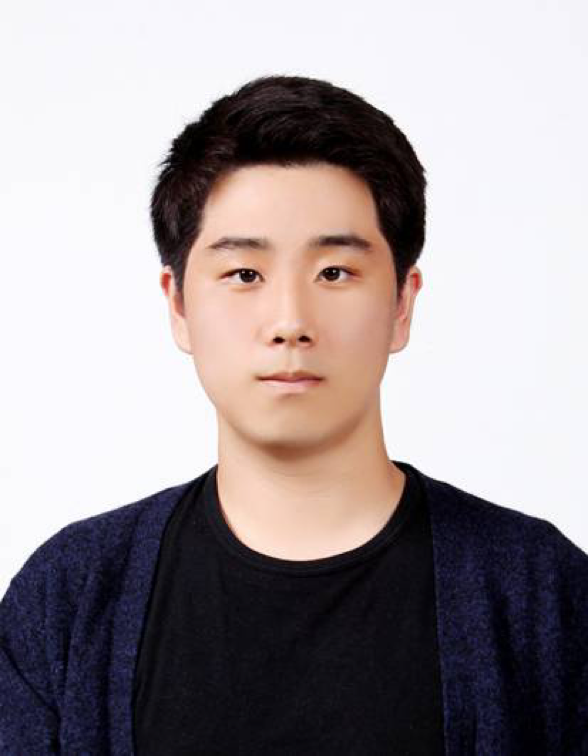
\includegraphics[width=1in,height=1.25in,clip,keepaspectratio]{author1.png}
}
\noindent
{\bf Sangsoo Lee} received his B.S. degree from Korea University, sejong, Korea. He is currently pursuing an M.S. degree in the Department of Mathematics at Sogang University, Seoul, Korea. His research interests include generative AI, image databases, and large language models (LLMs).\\
\noindent

\parpic[l]{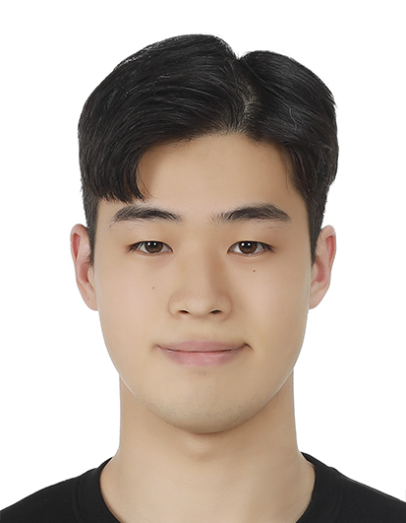
\includegraphics[width=1in,height=1.25in,clip,keepaspectratio]{author2.png}
}
\noindent
{\bf Jae-Hyun Baek} received his B.S. degree from Sogang University, Seoul, Korea. He is currently hoping to pursue an M.S. degree in the Department of Mathematics at Sogang University, Seoul, Korea. His research interests include Deep Learning, Image Analysis, large language models (LLMs), and AI security.\\

\parpic[l]{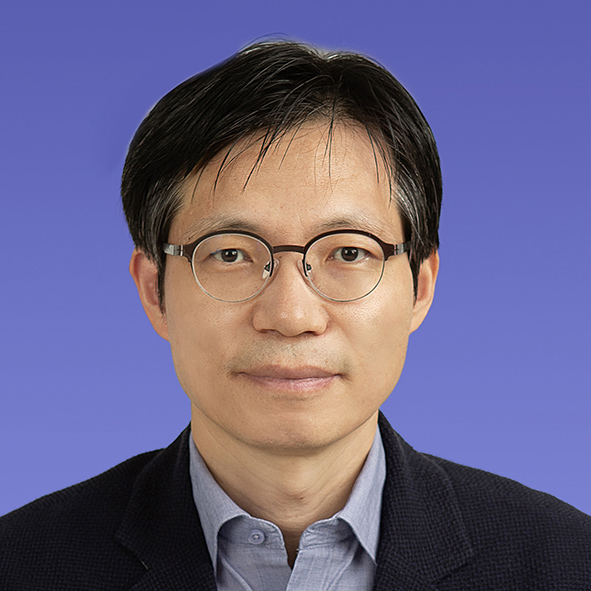
\includegraphics[width=1in,height=1.25in,clip,keepaspectratio]{Corresponding Author.jpg}
}
\noindent
{\bf Jon-Lark Kim} received his B.S. degree
in mathematics from Pohang University
of Science and Technology (POSTECH),
finished the master\textquotesingle s course in mathematics from Seoul National University, and
received his Ph.D. in mathematics from
the University of Illinois at Chicago, in 1993, 1997, and 2002,
respectively. He joined the University of Nebraska-Lincoln
from 2002 to 2005 as a research assistant professor. He joined
the University of Louisville between 2005 and 2012 as an assistant and association professor. Since 2012, he has been a
professor at the Department of Mathematics at Sogang University, Seoul, Korea. His research interests include coding theory,
cryptography, soft computing, and artificial intelligence.\\


\end{document}
